%\documentclass[xcolor=dvipsnames,9pt,hide notes]{beamer}
\documentclass[xcolor=dvipsnames,9pt,hide notes,mathserif]{beamer}

\usepackage{listings}
\definecolor{darkred}{rgb}{0.5,0,0}
\setbeamerfont{structure}{family=\rmfamily,shape=\scshape}
% \usecolortheme[name=darkred]{structure}

% \newcommand{\nat}{\ensuremath{\operatorname{nat}}}
\newcommand{\nat}{\ensuremath{\mathsf{nat}}}
% \newcommand{\bool}{\ensuremath{\operatorname{bool}}}
\newcommand{\bool}{\ensuremath{\mathsf{bool}}}
\newcommand{\alloc}{\ensuremath{\mathsf{alloc}}}
\newcommand{\emp}{\ensuremath{\mathsf{emp}}}
\newcommand{\heap}{\ensuremath{\mathsf{heap}}}
\newcommand{\this}{\ensuremath{\mathsf{this}}}
\newcommand{\mem}{\ensuremath{\mathsf{mem}}}
\newcommand{\hid}{\ensuremath{\mathsf{hid}}}
\newcommand{\upd}{\ensuremath{\mathsf{upd}}} 
\newcommand{\fix}{\ensuremath{\mathsf{fix}}} 
\newcommand{\eval}{\ensuremath{\mathsf{eval}}} 
% \renewcommand{\do}{\ensuremath{\mathsf{do}}} 
\newcommand{\diverge}{\ensuremath{\mathsf{diverge}}} 
\newcommand{\seleq}{\ensuremath{\mathsf{seleq}}} 
\renewcommand{\empty}{\ensuremath{\mathsf{empty}}} 
\newcommand{\splits}{\ensuremath{\mathsf{splits}}} 

\title[HTT]{A gentle introduction to Hoare Type Theory}

\author[Hyeyoung Shin]{Hyeyoung Shin\\
  {\small \url{hyeyoung@iastate.edu}}}
\institute[\url{hyeyoung@iastate.edul}]{%
  {\color{darkred}  {\small Iowa State University}}}
\date{6 July 2016}



\begin{document}

\maketitle 


\begin{frame}
  \frametitle{}
  Hoare Type Theory, Polymorphism and Separation (2007)
  \vskip1cm
  Nanevski, Morrisett and Birkedal
\end{frame}



\begin{frame}
  \frametitle{Problem}
  Errors not caught by today's type systems 
  \begin{itemize}
  \item array-index-out-of-bounds
  \item division-by-zero
  \end{itemize}
\vskip1cm
  and high-level correctness issues
  \begin{itemize}
  \item invariants
  \item protocols on mutable data structures
  \end{itemize}

\end{frame}



\begin{frame}
  \frametitle{Alternative Solutions}
  \begin{enumerate}
  \item dependent types
\vskip1cm
  \item program logics
    \begin{itemize}
    \item Hoare Logic
    \item Separation Logic
    \end{itemize}
  \end{enumerate}
\end{frame}




% \begin{frame}
%   \frametitle{Power of Dependent type}
%   sorting algorithm: 
%   \begin{itemize}
%   \item  $sort : List(\mathbb{N}) \rightarrow List(\mathbb{N})$
%   \item<2-> $sort : (n: \mathbb{N}) Vector(n) \rightarrow Vector(n)$
%   \item<3-> $sort: (n: \mathbb{N}) Vector(n) \rightarrow OrdVector(n)$
%     \\[4pt]
%     where $OrdVector(n) := (x_1 : \mathbb{N}) \times (x_2 :
%     \mathbb{N}_{x_1+1}) \times \dots \times (x_n :
%     \mathbb{N}_{x_{n-1}+1})$.
%   \end{itemize}
% \end{frame}






% \begin{frame}
%   \frametitle{Example: Dependent type}
%   OrdVector(4) = $(x_1: \mathbb{N}) \times (x_2: \mathbb{N}_{x_1+1})
%   \times (x_3 : \mathbb{N}_{x_2 + 1}) \times (x_4 :
%   \mathbb{N}_{x_3+1})$.
%   \vskip1cm
%   $<5, 3, 3, 0>$ is an element of this type because 
%   \begin{align*}
      %       &5: \mathbb{N}\\
      %               &3: \mathbb{N}_{5+1} = \mathbb{N}_6 = \{0,1,2,3,4,5\} \\
      %               &3: \mathbb{N}_{3+1} = \mathbb{N}_4 = \{0,1,2,3\} \\
      %               &0: \mathbb{N}_{3+1} = \mathbb{N}_4 = \{0,1,2,3\} \\
      %     \end{align*}
      %       \end{frame}







      %       \begin{frame}
      %       \frametitle{Example: Dependent type}
      %       OrdVector(4) = $(x_1: \mathbb{N}) \times (x_2: \mathbb{N}_{x_1+1})
      %       \times (x_3 : \mathbb{N}_{x_2 + 1}) \times (x_4 :
      %       \mathbb{N}_{x_3+1})$.
      %       \vskip1cm
      %       $<5, 3, 4, 0>$ is \textit{not} an element of this type because 
      %       \begin{align*}
      %               &5: \mathbb{N}\\
      %               &3: \mathbb{N}_{5+1} = \mathbb{N}_6 = \{0,1,2,3,4,5\}\\
      %               &4: \mathbb{N}_{3+1} = \mathbb{N}_4 = \{0,1,2,3\} \\
      %               &0: \mathbb{N}_{3+1} = \mathbb{N}_4 = \{0,1,2,3\}\\
      %     \end{align*}
      %       \end{frame}







\begin{frame}
  \frametitle{Hoare Logic}
  \textit{Hoare Triple}: $\{P\} C \{Q\}$
  \vskip1cm
  A reasoning system that can carry out \textit{program verification}
  well suited to imperative programs
  \begin{itemize}
  \item a natural way of writing down specifications of programs
  \item a \textit{compositional proof technique}
  \end{itemize}
\end{frame}








\begin{frame}
  \frametitle{Separation Logic}

An extension of Hoare's logic for specifying and verifying properties of dynamically-allocated linked data structure
\begin{itemize}
\item much simpler by-hand specification and program proofs
\end{itemize}

\vskip0.5cm

Specifications are ``small'': it concentrates on the resources relavant to its correct operations (its ``footprint'')

\vskip0.5cm

More specifically, during its execution, $c$ may access only memory locations whose existence is asserted in the precondition or that have been allocated by $c$ itself
  \begin{itemize} 
  \item \textit{local reasoning}
  \end{itemize}
\end{frame}




\begin{frame}
  \frametitle{$P \ast Q$: Separating conjunction}

$P$ and $Q$ hold for separate portions of memory and program-proof rules that exploit separation to provide modular reasoning about programs

  \begin{itemize} 
  \item \textit{local reasoning}
  \end{itemize}
  \vskip1cm
In addition to the standard Hoare logic rules, Separation logic supports\\
the frame rule:\\
  \[\underline{\phantom{XXXX} \{P\} C \{Q\} \phantom{XXXX}} \; \mathrm{mod}(C) \cap \mathrm{free}(R)=\emptyset\]
  \[ \{P \ast R\} C \{Q \ast R\} \phantom{XXXXXXXXXXXXX}\]

\vskip0.3cm
``none of the variables modified by C occur free in R''

\end{frame}



%% \begin{frame}
%%   \frametitle{Example of the Use of Separation Logic}
%%   disposing a tree:
%%   \begin{align*}
       %%        disptree(p) &[tree(p)] \{\\
       %%                              &local i,j;\\
       %%                              &if(p=nil) \{\} else \{\\
       %%                              &i := p \rightarrow l; j := p\rightarrow r; disptree(i);\\
       %%                              &disptree(j); disptree(p); \}\\
       %%                              &\} [emp]\\
       %%      \end{align*}
       %%        Partial correctness specification: $[tree(p)] disptree(p) [emp]$
       %%        \end{frame}





\begin{frame}
  \frametitle{Limitation of Previous work}
  \begin{enumerate}
  \item dependent types
    \begin{itemize}
    \item do not work well with side effects (state updates, non-termination)
    \end{itemize}
  \item program logics
    \begin{itemize}
    \item do not integrate \textit{into} the type system
    \item make it difficult to scale the logics to support the
      abstraction mechanisms (higher order functions, polymorphism,
      modules)
    \end{itemize}
  \end{enumerate}
\end{frame}











\begin{frame}
  \frametitle{Solution}
  \textbf{Hoare Type Theory}: Types with Hoare-style specifications
\end{frame}




\begin{frame}
  \frametitle{The Hoare Type}
  The key mechanism: Hoare Type constructor $\Psi.X.\{P\}x:A\{Q\}$ 
  \begin{itemize}
%  \item   when executed in a heap satisfying the precondition $P$, the
%    computation diverges or results in a heap satisfying the
%    postcondition $Q$ and returns a value of type $A$ in context $\Psi$
%    and $X$.
  \item Simultaneously isolates and describes the effects of imperative commands
  \item keeps track of the effectful computation in the dependent setting
    \begin{itemize}
    \item  refinement of the concept of \textit{monad}
    \item ``type marker'' for computations with side effects
    \end{itemize}
    \item can be nested, combined with other types, and abstracted
      within terms, types and predicates
\item provides a unified system for programming, specification and
  reasoning about programs
  \end{itemize}
\end{frame}

       %%        \begin{frame}
       %%        \frametitle{Monad}
       %%        \begin{center}
       %%        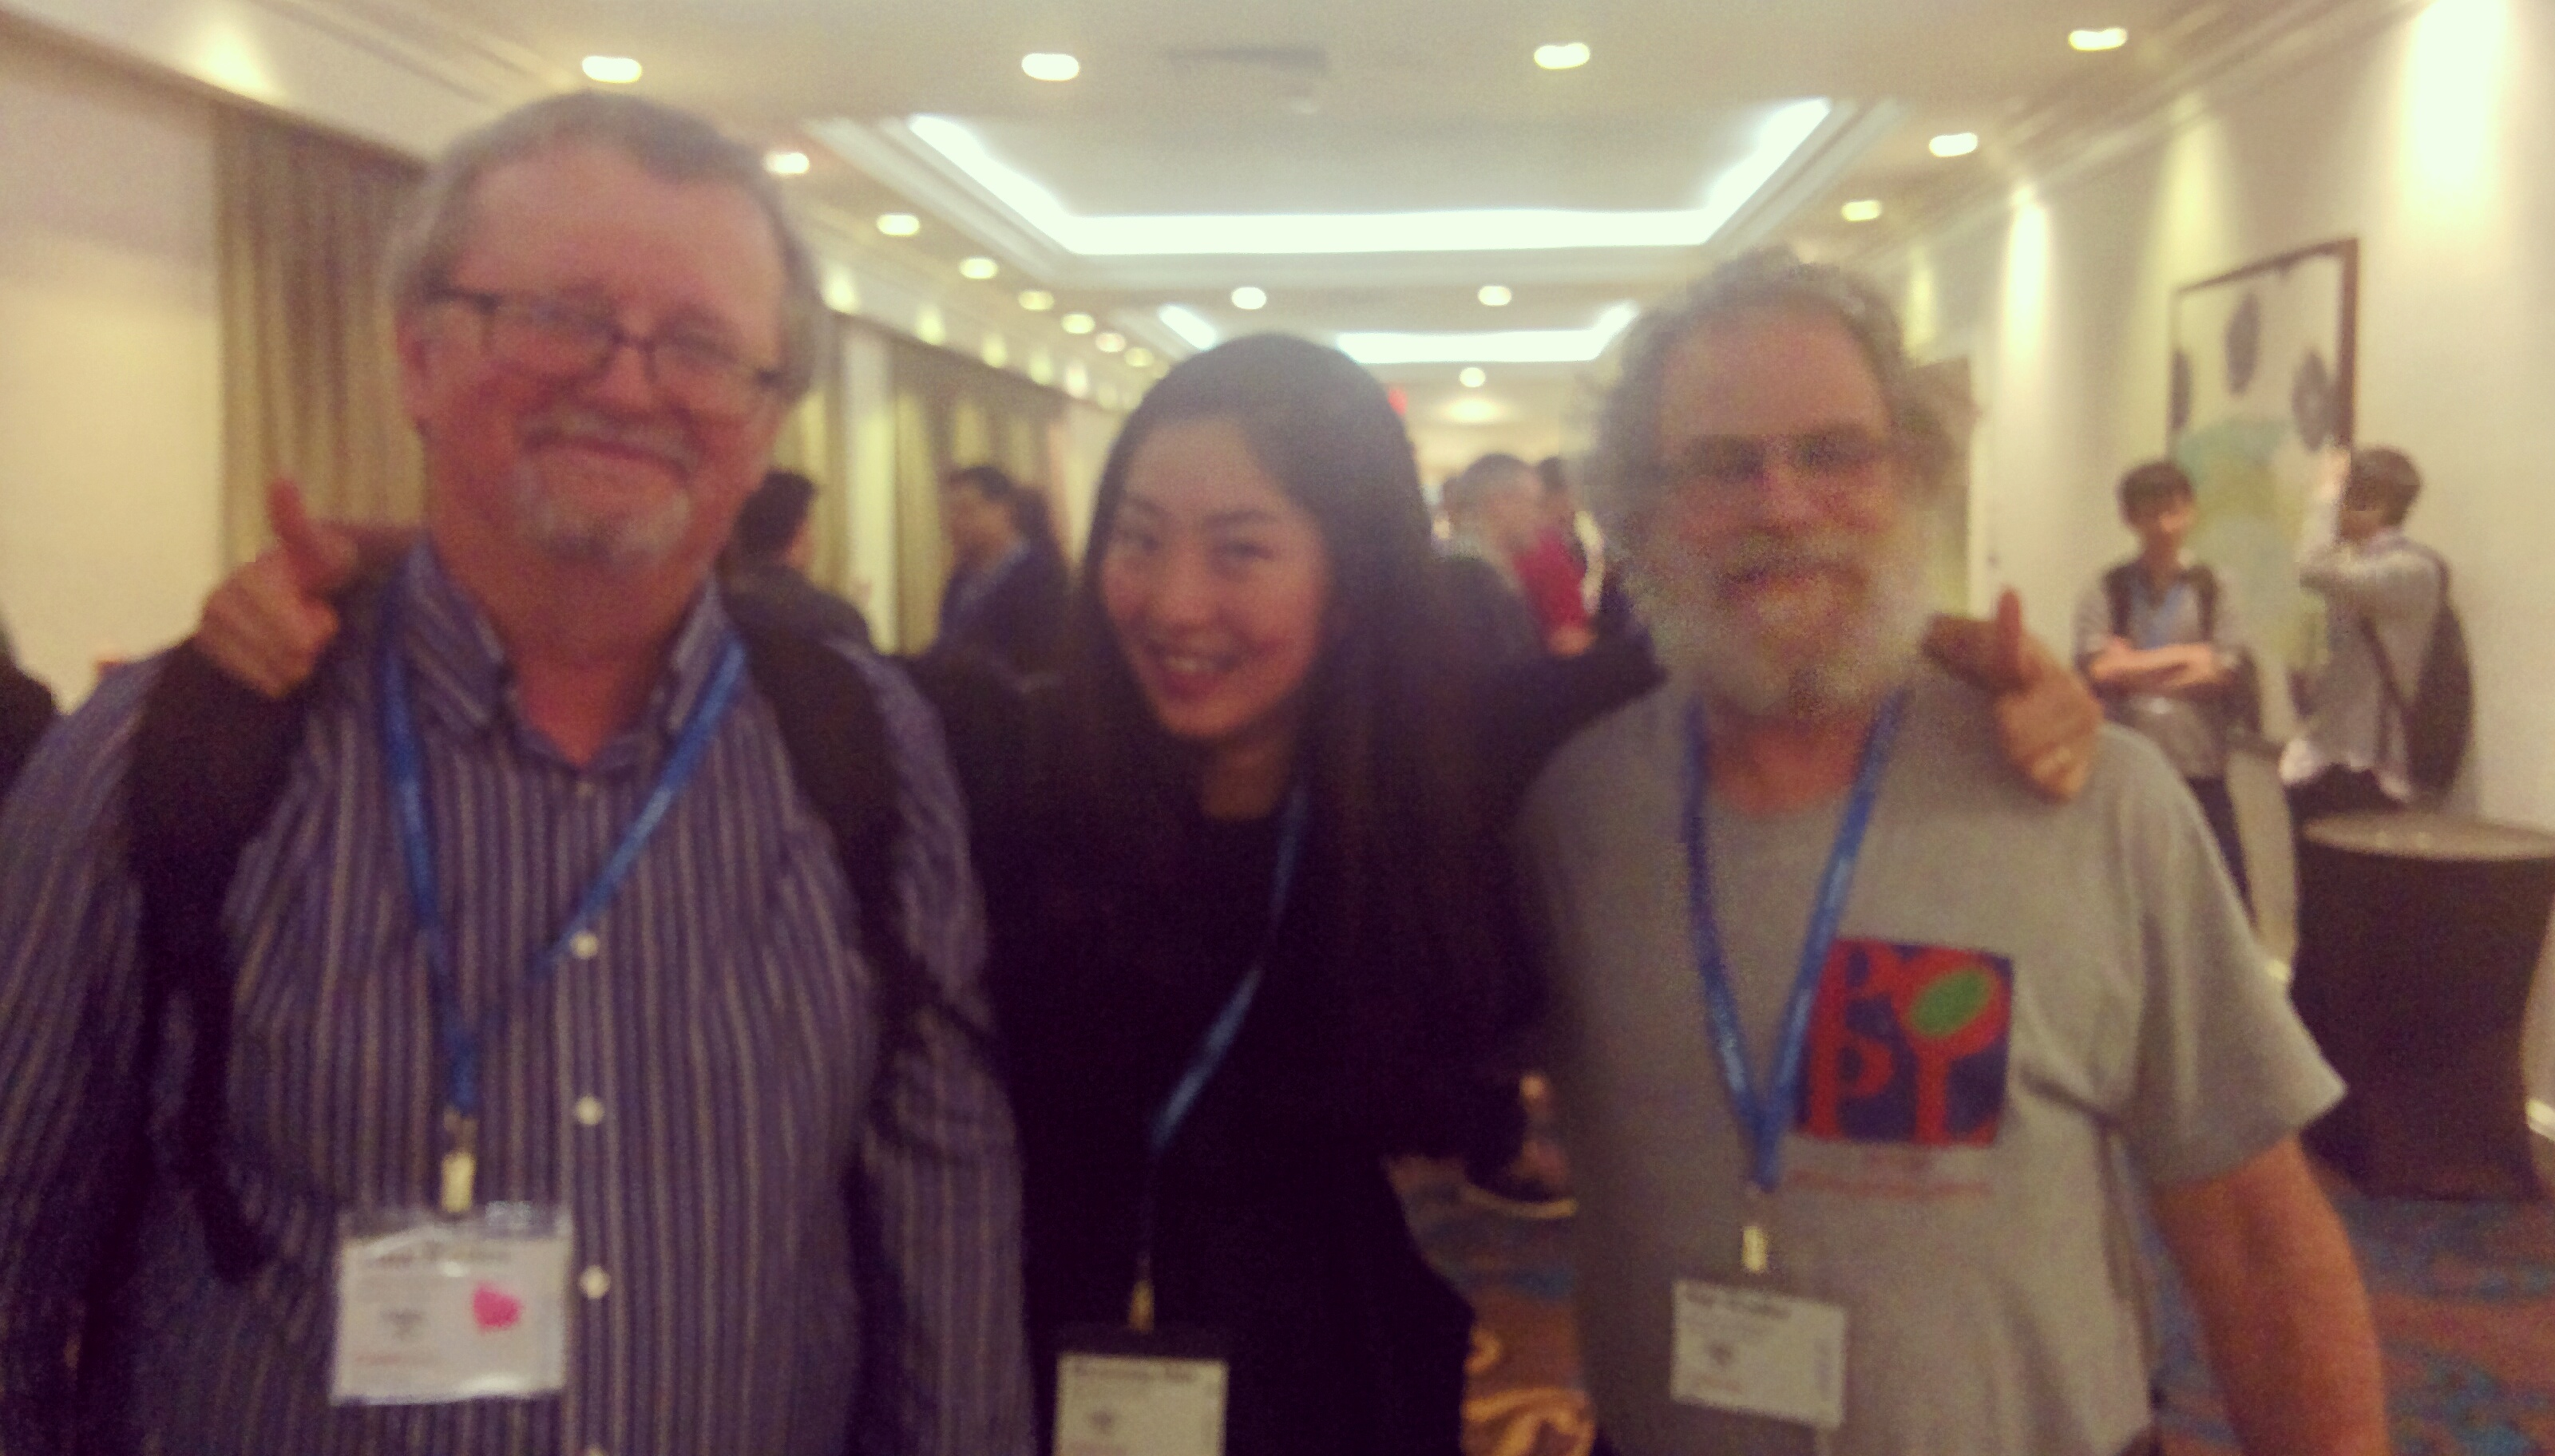
\includegraphics[width=10cm]{buddies}
       %%        \end{center}
       %%        John Hughes(left)  Philp Wadler(right)
       %%        \end{frame}

       %%        \begin{frame}
       %%        \frametitle{What is a Monad?}
       %%        \[809\]
       %%        \begin{quote}``what would be a brief, succinct, practical explanation
       %%        as to what a monad essentially is?''
       %%        \end{quote}
       %%        \[770\]
       %%        \end{frame}

       %%        \begin{frame}
       %%        \frametitle{What is a Monad?}
       %%        \begin{quote} ``I think monads are hard because nobody can seem to figure
       %%        out how to explain them without getting caught up in confusing
       %%        implementation details. I mean.. what is a school bus? It's a metal
       %%        platform with a device in the front which consumes a refined
       %%        petroleum product to drive in a cycle some metallic pistons, which
       %%        in turn rotate a crank shaft attached to some gears which drive some
       %%        wheels. The wheels have inflated rubber bags around them which
       %%        interface with an ashphalt surface to cause a collection of seats to
       %%        move forward. The seats move forward because...'' Breton 
       %%        \end{quote}
       %%        \end{frame}


       %%        \begin{frame}
       %%        \frametitle{Monad}
       %%        Maybe type
       %%        \vskip1cm
       %%        functor $\Rightarrow$ applicative functor $\Rightarrow$ Monad $\Rightarrow$ Hoare Type
       %%        \end{frame}


\begin{frame}
  \frametitle{Contents of the talk}
  \begin{enumerate} 
  \item Overview
  \item Syntax
    \begin{itemize}
    \item Terms
    \item Computations
    \item Types
    \item Heaps and locations
    \item Assertions
    \end{itemize}
  \item Type System
    \begin{itemize}
    \item Equational reasoning
    \item Typing rules
    \end{itemize}
  \item Hereditary substitutions
  \item Properties
  \item Operational semantics
    \begin{itemize}
    \item Preservation
    \item Progress
    \end{itemize}
  \item Heap soundness
  \end{enumerate}
\end{frame}










\begin{frame}
  \frametitle{1. Overview of HTT programs}
  \begin{itemize}
  \item the pure fragment
    \begin{itemize}
    \item higher-order functions
    \item constructs for type polymorphism
    \end{itemize}
  \item the impure fragment 
    \begin{itemize}
    \item allocation
    \item lookup
    \item strong update
    \item deallocation of memory
    \item conditional
    \item loops (recursion)
    \end{itemize}
  \end{itemize}
  \vskip1cm
  the Hoare type $\{P\}x:A\{Q\}$ classifies the impure programs
\end{frame}









\begin{frame}
  \frametitle{Example: Small and large footprints}

  % \begin{lstlisting}
% {\bf alloc}: $\forall \alpha. \Pi_x:\alpha$ \{emp\} {\bf y}:nat $\{\mathbf{y} \mapsto_\alpha \mathbf{x}\}$
  \[
   \alloc : \forall \alpha.\; \Pi x{:}\alpha\;  \{\emp \} y {:} \nat \{y \mapsto_\alpha x\}
 \]
  % \end{lstlisting}

  \begin{itemize}
  \item y must be fresh because \{emp\} prohibits alloc form working with existing locations
  \end{itemize}
  
\end{frame}

\begin{frame}
  \frametitle{Example: Small and large footprints}
\[
    \alloc': \forall \alpha.\; \Pi x{:}\alpha.\; z{:} \nat,  v{:} \bool. \;
    \{z \mapsto_{\bool} v\} y{:}\nat \{ y \mapsto_\alpha x \ast z \mapsto_{\bool} v\}
\]
  \begin{itemize}
  \item $z$ and $v$ denote the assumed existing location and its contents
  \item $\alloc'$ allows execution only in heaps with \textit{at least} one boolean location
  \item The specification insists that the contents of z is not changed by the execution
  \item $\ast$ specifies that $z$ and $v$ belong to disjoint heap portions, hence $y$ is fresh
  \end{itemize}
\end{frame}





\begin{frame}
  \frametitle{Example: Small and large footprints}

\[
   \alloc'': \forall \alpha. \; \Pi x {:} \alpha. \; h{:}\heap \{\this(h)\} y{:} \nat \{ (y \mapsto_\alpha x) * \this(h)\}
\]

  \begin{itemize}
  \item $\this(h) = \hid (\mem, H)$ ``heap equality''
  \item We can name the heap encountered before allocation using a ghost variable $h$    
  \end{itemize}

\end{frame}







\begin{frame}
  \frametitle{Example: Small and large footprints}

\[
   \alloc''': \forall \alpha. \; \Pi x {:} \alpha. \; h{:}\heap \{\this(h)\} y{:} \nat \{\this(\upd_\alpha(h,y,x) \wedge y \notin h\}
\]

  \begin{itemize}
  \item<1-> classical style (large footprint)
  \item<2-> By explicitly naming various heap fragments with ghost variables, HTT can freely switch from the small and large footprint specifications
  \end{itemize}

\end{frame}



% \end{document}



\begin{frame}
  \frametitle{}

  \begin{itemize}
  \item small specificaiton: convenient for programming
  \item large footprint: convenient in case aliasing is allowed
  \item naming of heap fragment: easy to connect to the assertion logic in HTT
  \end{itemize}

\end{frame}





\begin{frame}
  \frametitle{Example: Diverging computation}
\begin{align*}
    \diverge &: \{P\} x{:}A \{Q\} \\
   &= \mathsf{do} (\fix f(y{:}1) : \{P\} x{:}A \{Q\} = \mathsf{do} (\eval (f y))\\
    &\phantom{XXX}\mathsf{in} \; \eval f ())
\end{align*}

  \begin{itemize}
  \item non-termination is an effect (impure computation)
  \item do E: intro term for the Hoare type which encapsulates the effectful computation E and suspends its evaluation
  \item so {\bf diverge}, when forced, sets up a recursive function 
    f(y:1) = do (eval f(y)).
  \end{itemize}

\end{frame}





\begin{frame}
  \frametitle{2. Syntax}
\end{frame}







\begin{frame}
  \frametitle{Terms: the purely functional fragment of HTT}
  The separation into {\bf intro} and {\bf elim} terms facilitate \textit{bidirectional typing checking} (Pierce \& Turner. 2000)
\end{frame}






\begin{frame}
  \frametitle{Computations: the effectful fragment of HTT}
  Semicolon-separated lists of commands, terminated with a return type\\
  The commands are executed in the order of the list and usually bind their result to a variable\\
  Variables in HTT are immutable unlike those of Hoare logic
\end{frame}




\begin{frame}
  \frametitle{Commands}
\end{frame}






\begin{frame}
  \frametitle{Types}
  \begin{itemize}
  \item the primitive types: booleans and nats
  \item unit type: 1
  \item the Hoare type: $\Psi.X.\{P\}x:A\{Q\}$
  \item dependent function type: $\Pi_{x:A} B(x)$
  \item polymorphic type: $\forall \alpha.A$
  \end{itemize}
  
\end{frame}






\begin{frame}
  \frametitle{The Hoare Type: $\Psi.X.\{P\}x{:}A\{Q\}$}
  \begin{itemize}
  \item specifies an effectful computation with precondition P and postcondition Q returning a result of type A
  \item x: the name of the return type
  \item Q may depend on x
  \item $\Psi$ lists the variables
  \item X lists the heap variables  (ghost variables: only appear in the assertions, not in the program)
  \end{itemize}
  
\end{frame}






\begin{frame}
  \frametitle{Dependent function type: $\Pi x{:}A. B$}
  a.k.a forall type or product type

\[
  f: A \rightarrow \bigcup_{a:A} B(a)  \quad\text{ and }\quad \forall a \in A. f(a) \in B(a)
\]
\vskip1cm
This is equivalent to the more concise notation
\[
  f:  \prod_{a{:}A}B(a)
\]
\vskip1cm
For example, if $A = \{0,1,2\}$, then $\Pi x{:}A.B(x) = B(0) \times B(1) \times B(2)$.
\end{frame}



\begin{frame}
  \frametitle{Polymorphic type: $\forall \alpha.A$}
  polymorphically quantifies over the monotype variable $\alpha$
  
  \begin{itemize}
  \item \textit{monotype} in HTT: any type that does not contain polymorphic quantification, except in assertions
    $\Rightarrow$ \textit{predicative} polymorphism (range of type variable is restricted to monotypes)
  \end{itemize}
\vskip1cm
  Extending HTT to support \textit{impredicative} polymorphism is left for future work since it significantly complicates the termination argument for normalization (e.g. X in T = $\forall X. X \rightarrow X$ ranges over all types, including T itself)
  
\end{frame}






\begin{frame}
  \frametitle{Heaps and locations}
  Memory locations as natural number to support pointer arithmetic\\
  Heaps as finite functions\\[6pt]

  $N \longrightarrow (\tau, M)$\\[6pt]

  ``N points to M'' or ``M is the contents of location N''
  
  \begin{itemize}
  \item empty
  \item $\upd_\tau$ (H, M, N)
  \end{itemize}

\end{frame}








\begin{frame}
  \frametitle{Assertions: from classical first order logic}
  \begin{itemize}
  \item $id_A(M,N)$
  \item $\seleq_\tau(H, M, N)$ : the heap H at address M contains a term N:$\tau$
  \item $P \supset \subset Q$ : $P \supset Q \wedge Q \supset P$
  \item $\hid(H_1, H_2)$ : the heap equality
  \item $M \in H$ : M assigns the location M 
  \item $M \notin H$
  \item share($H_1, H_2, M$) : $H_1$ and $H_2$ agree on the location M
  \item splits($H, H_1, H_2$) : $H$ can be split into disjoint heaps $H_1$ and $H_2$
  \end{itemize}
\end{frame}




\begin{frame}
  \frametitle{Assertions: from Separation logic}
Free variable {\bf mem} denotes the current heap fragment
  \begin{itemize}
  \item $\emp = \hid(\mem,\empty)$
  \item $M \mapsto_\tau N = \hid(\mem, \upd_\tau(\empty, M, N))$
  \item $M \mapsto_\tau - = \exists v{:} \tau.\; M \mapsto_\tau v$
  \item $M \mapsto - = \exists \alpha.\; M \mapsto_\alpha -$
  \item $M \hookrightarrow_\tau N = \seleq_\tau(\mem, M,N)$
  \item $M \hookrightarrow_\tau - = \exists v{:}\tau.\; M \hookrightarrow_\tau v$
  \item $M \hookrightarrow - = \exists \alpha. \;M \hookrightarrow_\alpha -$
  \item $P \ast Q = \exists h_1: \heap, \exists h_2:\heap. \;
    \splits(\mem, h_!, h_2) \wedge [h_1/\mem] P \wedge [h_2/\mem]Q$
  \item $P -\ast Q = \forall h_1, \forall h_2. \splits(h_2, h_1, \mem) \supset [h_1/\mem] P \supset [h_2/\mem]Q$
  \end{itemize}
\end{frame}






\begin{frame}
  \frametitle{3.Type System}
  Type checking judgements require testing if two terms are definitionally equal and testing definitional equality involves normalization.


    \begin{itemize}
    \item Two terms are equal only if the canonical forms are syntactically the same, modulo $\alpha$-conversion
    \item Unusual in HTT: normalization is undertaken \textit{simultaneously} with type checking 
    \end{itemize}

\end{frame}







\begin{frame}
  \frametitle{3.1 Equational reasoning}
Beta and eta equalities are most important in HTT definitional equality

What's Unusual in HTT? Normalization is undertaken \textit{simultaneously} with type checking 

\end{frame}


%\end{document}


\begin{frame}
  \frametitle{Equations for}

    \begin{itemize}
    \item $\Pi x{:}A.B$
\begin{align*}
(\lambda x.M : \Pi x{:}A.B)N &\longrightarrow_\beta [N{:}A/x]M\\
                                         K &\longrightarrow_\eta \lambda x.K x     \quad    x \notin FV(K) 
\end{align*}
    \item $\forall \alpha.A$
\begin{align*}
(\Lambda \alpha.M : \forall \alpha. A)\tau &\longrightarrow_\beta [\tau/\alpha]M\\
                                         K &\longrightarrow_\eta \Lambda \alpha.K \alpha     \quad    \alpha \notin FTV(K) 
\end{align*}
\item 1
\[
K \longrightarrow_\eta ()
\]
    \end{itemize}

\end{frame}


\begin{frame}
  \frametitle{Equations for the Hoard type}
requires an auxiliary operation of monadic substitution
\[
\langle E/x{:}A \rangle F,
\]
which subsequently composes the computations E and F, `` E followed by F'',
and free variable $x{:}A$ in F is bound to the value of E.

\vskip1cm
Monadic substitution is defined by induction on the structure of E.


\begin{align*}
x \longleftarrow (\mathrm{do} E : \{P\} x{:}A \{Q\}); F &\longrightarrow_\beta \langle E/x{:}A \rangle F\\
                                         K &\longrightarrow_\eta \mathrm{do} (x \longleftarrow K; return x)
\end{align*}

\end{frame}






\begin{frame}
  \frametitle{Normalization algorithm}
uses specific expand (\textit{expand$_A$}) and reduction (\textit{hereditary substitution}) strategy.

\begin{itemize}
\item expand$_A$ iterates over the type A and expands the given argument (elim or intro term) according to each encountered type constructor
\item hereditary substitution operates on canonical terms only (e.g. whenever an ordinary capture avoiding substitution creates a redex like $(\lambda x.M)N$, hereditary substitution continues by immediately substituting N for $x$ in M)
\end{itemize}

\end{frame}




\begin{frame}
  \frametitle{Normalization algorithm}
uses specific expand (\textit{expand$_A$}) and reduction (\textit{hereditary substitution}) strategy.

\begin{itemize}
\item expand$_A$ iterates over the type A and expands the given argument (elim or intro term) according to each encountered type constructor
\item hereditary substitution operates on canonical terms only (e.g. whenever an ordinary capture avoiding substitution creates a redex like $(\lambda x.M)N$, hereditary substitution continues by immediately substituting N for $x$ in M)
\end{itemize}

\end{frame}








\begin{frame}
  \frametitle{3.2 Typing rules}
  \textit{Undecidable}
  \begin{enumerate}
  \item basic type-checking and verification-condition generation
    \begin{itemize}
    \item completely automatic
    \end{itemize}
  \item validate the generated verification-conditions
    \begin{itemize}
    \item can be fed into an automated theorem prover
    \item can be discharged by hand
    \item can be ignored
    \end{itemize}
  \end{enumerate}
\end{frame}







\begin{frame}
  \frametitle{HTT vs. dependent types}
  \begin{itemize}
  \item When HTT was invented, some 10 years ago, dependent types were generally considered as
    being limited to the purely-functional and terminating programming
    model. 
    \item So it was a bit of a surprise that we could combine
      dependent types with dynamic state (i.e., pointers), and general
      recursion. (Amazingly, nobody had tried the idea before, in the
      dependently-typed setting.)
    \item  Even these days, when people do Hoare logic in a proof assistant such as Coq, most of the time they use deep embedding, which, while certainly expressive, results in proofs that are consider to be torture. 
  \end{itemize}
\end{frame}






\begin{frame}
  \frametitle{HTT vs. Hoare logic (or Separation logic)}
  \begin{itemize} 
 \item At the time HTT was invented, Separation logic was a
   first-order theory, incapable of reasoning about function calls,
   let alone abstract types, modules, objects, callbacks, etc.
\item  All of these come for free in HTT, as they are all instances of
  the $\Pi$ and $\Sigma$ types. (see ICFP'08 paper on the
  implementation of HTT, for a number of examples that are
  higher-order in this sense, and use the combination of dependent
  types with pre- and post-conditions, in an essential way)
\item Moreover, stack variables in Hoare logic are quite a
  complication, which is avoided in HTT, by means of the monadic
  formulation. 
\item Thus, monadic formulation made proofs much easier, as it
  eliminated pesky sidevconditions related to stack variables. 
\item Since then, higher-order versions of separation logic have been
  formulated, not by using dependent types, but still using monads. 
\item They are basically on the spectrum between ordinary separation
  logic and HTT, i.e., HTT is the logical limit of the idea. 
  \end{itemize}
\end{frame}





\begin{frame}
  \frametitle{HTT!}
It's usefulness lies in being able to structure your proofs in an easy and natural way, rather than in what can be technically done in it, compared to other systems.
\end{frame}





\begin{frame}
  \frametitle{6. Operational semantics}
call-by-value, left-to-right operational semantics
\vskip1cm
  \begin{itemize}
  \item if $\Delta; P \vdash E \Leftarrow x{:}A. Q$ is derivable in
    the type system, then it is the case that evaluating $E$ in a heap
    in which $P$ holds produces a heap in which $Q$ holds (if $E$ terminates).
    \item only defined for well-typed terms
  \end{itemize}
\end{frame}








\begin{frame}
  \frametitle{Syntax}
\begin{center}
    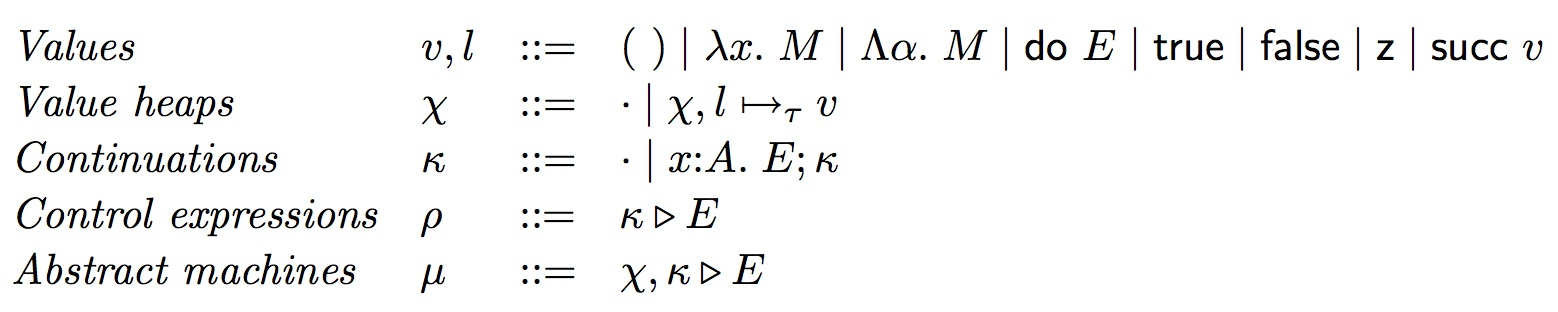
\includegraphics[width=10cm, height=3cm]{inputs/operational_syntax_htt}
\end{center}
\end{frame}






\begin{frame}
  \frametitle{Syntax}
\begin{center}
    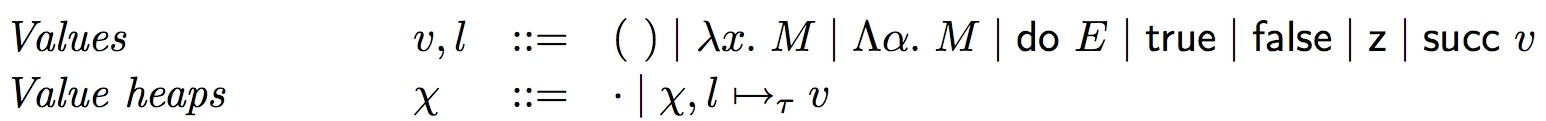
\includegraphics[width=10cm, height=1cm]{inputs/vv}
\end{center}
\begin{itemize}
\item {\bf values}: we use $l$ to range over nats when they are used as
  pointers
\item {\bf value heaps}: assignments from nats to values, where each
  assignment is indexed by a type
\begin{itemize}
\item run-time concept
\item used in the evaluation judgements to describe the state in which
  programs execute
\item note that heaps mentioned earlier are different and used for
  reasoning in the assertion logic
\end{itemize}
\begin{itemize}
\item two notions of heaps correspond to each other $\Rightarrow$
  \textit{heap soundness}
\end{itemize}
\end{itemize}
\end{frame}







\begin{frame}
  \frametitle{Syntax}
\begin{center}
    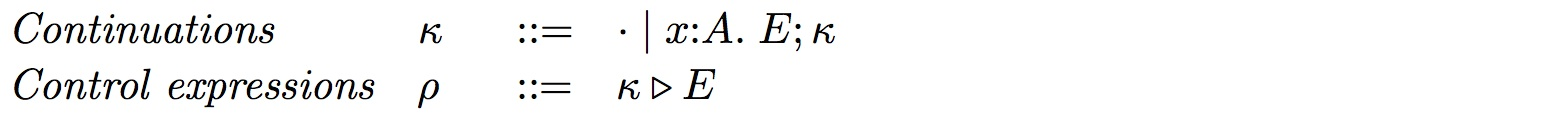
\includegraphics[width=10cm, height=1cm]{inputs/cc}
\end{center}
\begin{itemize}
\item {\bf continuation}: sequence of computations of the form
  $x{:}A. E$, where $E$ may depend on the bound variable $x{:} A$

\item {\bf control expression}: pairs up a computation $E$ and a
  continuation $k$ so that $E$ provides the initial value with which
  the execution $k$ can start 
\begin{itemize}
\item self-contained computation
\item makes the call-by-value semantics of the computation $x
  \leftarrow \do E; F$ explicit
\item evaluation of this computation is carried out by creating the
  control expression $x.F \rhd E;$ \\
``push $x.F$ on to the continuation and proceed to evaluate $E$''
\end{itemize}
\end{itemize}
\end{frame}







\begin{frame}
  \frametitle{Syntax}
\begin{center}
    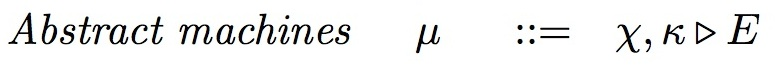
\includegraphics[width=5cm, height=0.5cm]{inputs/a}
\end{center}
\begin{itemize}
\item {\bf abstract machine}: a pair of a value heap $X$ and a control
  expression $k \rhd E$
\begin{itemize}
\item evaluated against the heap, to eventually produce a result and
  possibly change the heap
\end{itemize}
\end{itemize}
\end{frame}





\begin{frame}
  \frametitle{Evaluation}
\begin{center}
  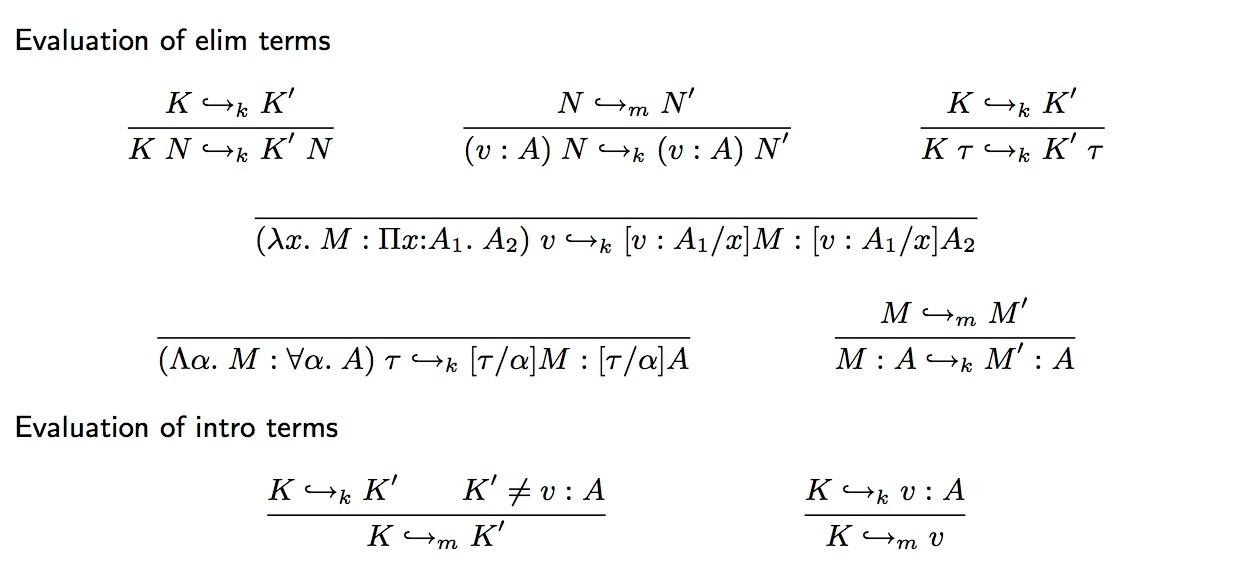
\includegraphics[width=10cm, height=5cm]{inputs/eval_elim_intro}
\end{center}
\end{frame}




\begin{frame}
  \frametitle{Evaluation}
\begin{center}
  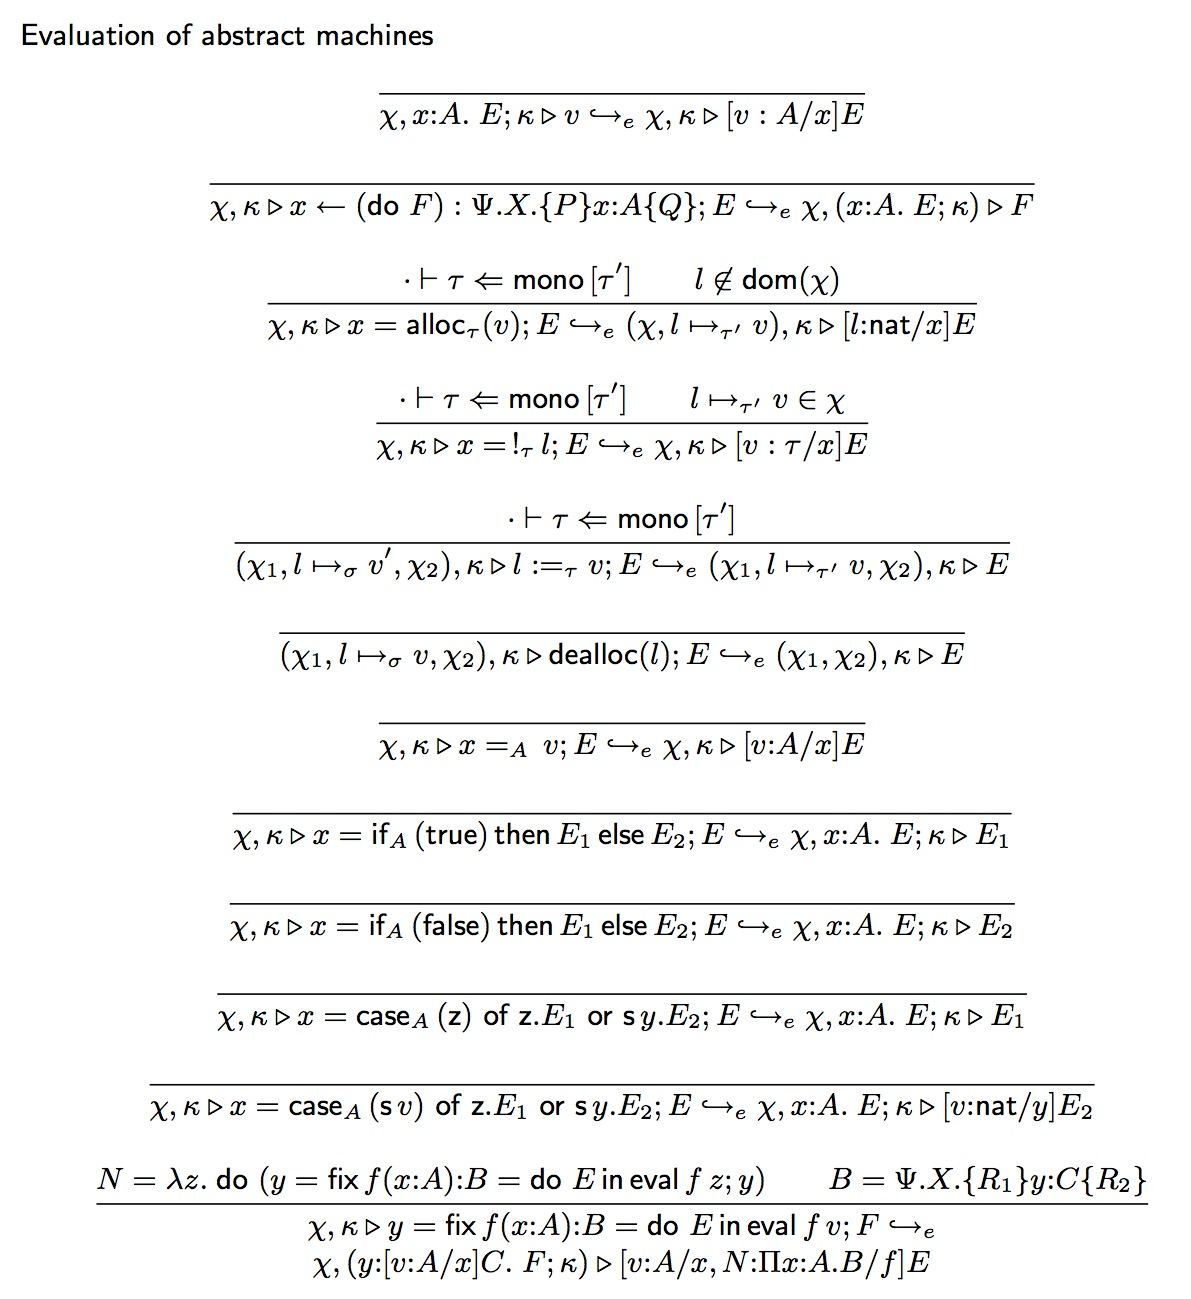
\includegraphics[width=10cm, height=8cm]{inputs/eval_abs}
\end{center}
\end{frame}





\begin{frame}
  \frametitle{Soundness}
via Preservation and Progress theorems
\begin{center}
  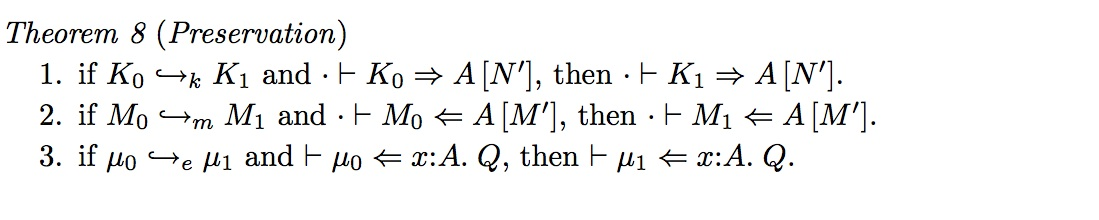
\includegraphics[width=13cm, height=3cm]{inputs/preservation}
\end{center}
\textit{Proof.} By induction on the evaluation judgement, using inversion
on the typing derivation, and substituting principles

\end{frame}





\begin{frame}
  \frametitle{Soundness}
\begin{center}
 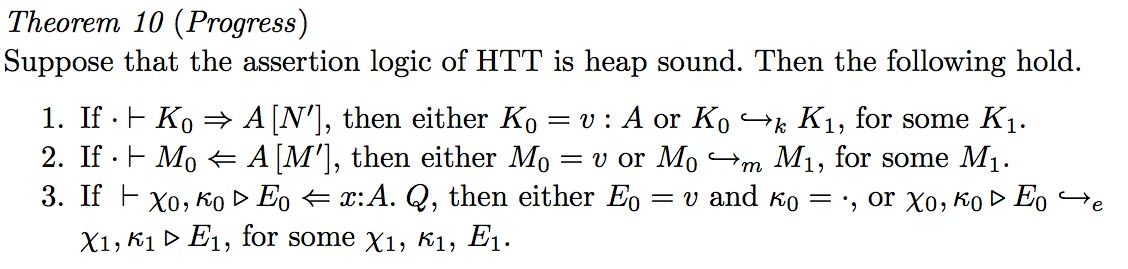
\includegraphics[width=11cm, height=3cm]{inputs/progress}
\end{center}
\textit{Proof.} By straightforward case analysis on the involved
expressions, employing inversion on the typing derivations, and the
proof of the third statement requires heap soundness 


\end{frame}



\begin{frame}
  \frametitle{Heap soundness}
\begin{center}
  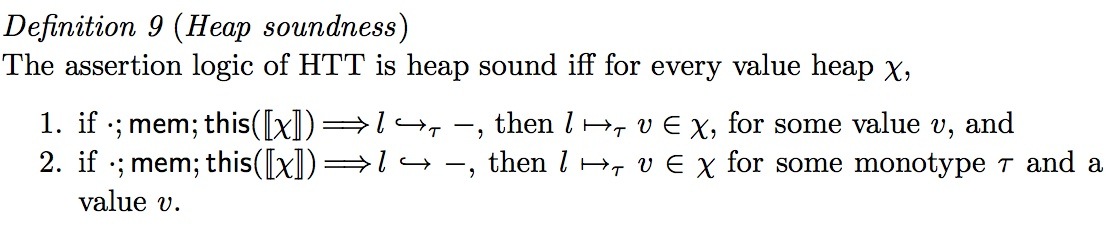
\includegraphics[width=11cm, height=2.5cm]{inputs/heap_soundness}
\end{center}

\textit{Theorem (Heap Soundness)}\\
The assertion logi of HTT is heap sound.
\vskip0.3cm

\textit{Proof.} refer to the paper
\end{frame}


\end{document}


\begin{frame}
  \frametitle{Soundness and Compositionality}
  Compositionality
  \begin{itemize}
  \item separate verifications of individual program ensures the
    correctness of the composite program
  \end{itemize}
  \vskip1cm
  Soundness
  \begin{itemize}
  \item types of HTT are strong
  \item verification does \textit{not} require whole-program reasoning
  \item \textit{Preservation} and \textit{Progress} theorem (at the end)
  \end{itemize}
\end{frame}





      %       \begin{frame}
      %       \frametitle{Type system}

      %       \end{frame}


      %       \begin{frame}
      %       \frametitle{Properties}

      %       \end{frame}

      %       \begin{frame}
      %       \frametitle{Operational semantics}

      %       \end{frame}




      %       \begin{frame}
      %       \frametitle{Preservation}
      %       \begin{enumerate}
      %       \item if $K_0 \hookrightarrow_k K_1$ and $\cdot \vdash K_0 \Rightarrow
      %       A[N']$, then $\cdot \vdash K_1 \Rightarrow A[N']$.
      %       \item if $M_0 \hookrightarrow_m M_1$ and $\cdot \vdash M_0 \Leftarrow
      %       A[M']$, then $\cdot \vdash M_1 \Rightarrow A[M']$.
      %       \item if $\mu_0 \hookrightarrow_e \mu_1$ and $\vdash \mu_0 \Leftarrow
      %       x:A. Q$, then $\vdash \mu_1 \Leftarrow x:A. Q$.
      %       \end{enumerate}
      %       \end{frame}




      %       \begin{frame}
      %       \frametitle{Progress}

      %       \end{frame}
      %       \begin{frame}
      %       \frametitle{Semantics of Program heaps in HTT}
      %       Functional arrays approach with Separation logic
      %       \begin{enumerate}
      %       \item Use of functional arrays 
      %       \begin{itemize}
      %       \item to define the connectives from Separation Logic in the presence of type polymorphism
      %       \end{itemize}
      %       \item ``small footprint'' idea from Separation logic 
      %       \begin{itemize}
      %       \item [$P$]$C$[$Q$]: if $C$ is given a heaplet satisfying $P$, then it will never try to access heap outside $P$ and it will deliver a heaplet satisfying $Q$ if it terminates 
      %       \end{itemize}
      %       \end{enumerate}
      %       \end{frame}













      %       \begin{frame}
      %       \frametitle{Syntax of HTT}
      %       \textbf{Equational reasoning}
      %       Type equality requires (undecidable) term equality in the case of dependent types
      %       \begin{itemize}
      %       \item \textit{definitional equality} provides decidability
      %       \begin{itemize}
      %       \item coarse but decidable
      %       \item employed during type-checking
      %       \end{itemize}
      %       \item \textit{propositional equality} provides preciseness
      %       \begin{itemize}
      %       \item fine but undecidable
      %       \item used only in proving
      %       \end{itemize}
      %       \end{itemize}
      %       \end{frame}






      %       \begin{frame}
      %       \frametitle{Syntax of HTT}
      %       \textbf{The split between pure and impure fragments}
      %       to separate the concerns about equality

      %       \begin{itemize}
      %       \item \textit{Pure} fragment admits the usual term equations of beta reduction and eta expansion
      %       \begin{itemize}
      %       \item higher-order functions
      %       \item constructs for type polymorphism
      %       \end{itemize}
      %       \item \textit{Impure} fragment admits reasoning in the style of Hoare Logic by pre- and post conditions
      %       \begin{itemize}
      %       \item constructs found in first-order imperative languages
      %       \begin{itemize}
      %       \item allocation 
      %       \item lookup 
      %       \item strong update
      %       \item deallocation of memory
      %       \item conditionals 
      %       \item loops(recursion)
      %       \end{itemize}
      %       \end{itemize}
      %       \end{itemize}
      %       \end{frame}



















\begin{frame}
  \frametitle{Example: Small and large footprints}

  \begin{lstlisting}
    {\bf alloc}: \forall \alpha. \Pi_x:\alpha \{emp\} {\bf y}:nat \{{\bf y} \mapsto_\alpha {\bf x}\}
  \end{lstlisting}

  \begin{itemize}
  \item y must be fresh because \{emp\} prohibits alloc form working with existing locations
  \end{itemize}
  
\end{frame}


\begin{frame}
  \frametitle{Example: Small and large footprints}

  \begin{lstlisting}
    {\bf alloc'}: \forall \alpha. \Pi_x:\alpha. {\bf z}:nat, {\bf v}:bool. \{{\bf z} \mapsto_{bool} {\bf v}\} {\bf y}:nat \{{\bf y} \mapsto_\alpha {\bf x} * {\bf z} \mapsto_{bool} {\bf v}\}
  \end{lstlisting}

  %% \begin{itemize}
  %% \item M \mapsto_\tau N iff {\bf mem} consists of a \emph{single} location M which points to the term N:\tau
  %% \end{itemize}

  \begin{itemize}
  \item {\bf z} and {\bf v} denote the assumed existing location and its contents
  \item {\bf alloc'} allows execution only in heaps with \emph{at least} one boolean location
  \item The specification insists that the contents of z is not changed by the execution
  \item * specifies that {\bf z} and {\bf v} belong to disjoint heap portions, hence {\bf y} is fresh
  \end{itemize}
  
\end{frame}





\begin{frame}
  \frametitle{Example: Small and large footprints}

  \begin{lstlisting}
    {\bf alloc''}: \forall \alpha. \Pi_x:\alpha. {\bf h}:heap \{this({\bf h})\} {\bf y}:nat \{{\bf y} \mapsto_\alpha x * this({\bf h})\}
  \end{lstlisting}

  \begin{itemize}
  \item this({\bf h}) = hid ({\bf mem}, H) ``heap equality''
  \item We can name the heap encountered before allocation using a ghost variable {\bf h}    
  \end{itemize}

\end{frame}








\begin{frame}
  \frametitle{Example: Small and large footprints}

  \begin{lstlisting}
    {\bf alloc'''}: \forall \alpha. \Pi_x:\alpha. {\bf h}:heap \{this({\bf h})\} {\bf y}:nat \{this(upd_\alpha(h,y,x) \wedge y \notin h\}
  \end{lstlisting}

  \begin{itemize}
  \item classical style (large footprint)
  \end{itemize}

\end{frame}







\begin{frame}
  \frametitle{Example: Small and large footprints}

  \begin{lstlisting}
    {\bf alloc'''}: \forall \alpha. \Pi_x:\alpha. {\bf h}:heap \{this({\bf h})\} {\bf y}:nat \{this(upd_\alpha(h,y,x) \wedge y \notin h\}
  \end{lstlisting}

  \begin{itemize}
  \item classical style (large footprint)
  \item By explicitly naming various heap fragments with ghost variables, HTT can freely switch from the small and large footprint specifications
  \end{itemize}

\end{frame}




\begin{frame}
  \frametitle{}

  \begin{itemize}
  \item small specificaiton: convenient for programming
  \item large footprint: convenient in case aliasing is allowed
  \item naming of heap fragment: easy to connect to the assertion logic in HTT
  \end{itemize}

\end{frame}





\begin{frame}
  \frametitle{Example: Diverging computation}

  \begin{lstlisting}
    {\bf diverge}: \{P\} x:A \{Q\} \\
    = do (fix f(y:1) : \{P\} x:A \{Q\} = do (eval f y))\\
    in eval f ())
  \end{lstlisting}

  \begin{itemize}
  \item non-termination is an effect (impure computation)
  \item do E: intro term for the Hoare type which encapsulates the effectful computation E and suspends its evaluation
  \item so {\bf diverge}, when forced, sets up a recursive function f(y:1) = do (eval f(y))
  \end{itemize}

\end{frame}



       %%        \begin{frame}
       %%        \frametitle{Types}
       %%        Booleans, natural numbers, unit type, dependent functions $\Pi x:A.B$,
       %%        and polymorphic types $\forall \alpha.A$
       %%        \vskip1cm
       %%        The Hoare type $\Psi.X.\{P\}x:A\{Q\}$
       %%        \begin{itemize}
       %%        \item specifies an effectful computation with a precondition $P$
       %%        and a postcondition $Q$, returning a result of type $A$
       %%        \item The variable $x$ names the return value of the computation
       %%        \end{itemize}

       %%        The context helps relate the properties of the beginning and the
       %%        ending heap
       %%        \begin{itemize}
       %%        \item $\Psi$ lists the variables
       %%        \item $X$ list the heap variable
       %%        \end{itemize}
       %%        \end{frame}











       %%        \begin{frame}
       %%        \frametitle{Hoare Type Theory}
       %%        main features
       %%        \begin{enumerate}
       %%        \item small footprint interpretation
       %%        \item monadic isolation
       %%        \item type polymorphism
       %%        \end{enumerate}
       %%        \end{frame}












       %%        \begin{frame}
       %%        \frametitle{1. Small Footprint semantics}
       %%        Hoare's original logic
       %%        \begin{itemize}
       %%        \item  pre- and post condition usually describes \textbf{the whole heap}
       %%        \begin{itemize}
       %%        \item cumbersome
       %%        \end{itemize}
       %%        \end{itemize}
       %%        \vskip1cm
       %%        HTT
       %%        \begin{itemize}
       %%        \item Talks only about \textbf{the portion of the heap relevant} to the correct
       %%        operation of the procedure (Separation Logic)
       %%        \item naming and manipulating individual fragments of the heap is
       %%        possible in the presence of type polymorphism (HTT)
       %%        \item supports \textbf{strong updates}
       %%        \end{itemize}
       %%        \end{frame}










       %%        \begin{frame}
       %%        \frametitle{Syntax of HTT 1}
       %%        Types
       %%        \[\dots \mid \forall \alpha.A \mid \Pi x:A.B \mid \Psi.X.\{P\} x:A
       %%        \{Q\}\]
       %%        Heap
       %%        \[ upd_\tau (H,M,N) \]
       %%        Assertions
       %%        \begin{align*}
       %%                              & P \subset \supset Q = P \supset Q \wedge Q \subset P\\
       %%                              & hid(H_1, H_2) = \forall \alpha. \forall x:nat. \forall
                                         %%                                          v:\alpha. seleq_\alpha (H_1, x, v) \subset \supset seleq_\alpha(H_2,
                                         %%                                          x,v)\\
       %%                              &emp = hid(mem, empty)\\
       %%                              &M \mapsto_\tau N = hid(mem, upd_\tau(empty,M,N))\\
       %%      \end{align*}
       %%        where \textbf{mem} is the current heap fragment
       %%        \end{frame}


       %%        \begin{frame}
       %%        \frametitle{Example: Specifications of HTT allocation primitive}
       %%        \[alloc: \forall \alpha. \Pi x:\alpha. \{emp\} y:nat \{y
       %%        \mapsto_\alpha x \} \]
       %%        \end{frame}

       %%        \begin{frame}
       %%        \frametitle{Example: Specifications of HTT allocation primitive}
       %%        \begin{align*}
       %%                              &alloc': \forall \alpha. \Pi x:\alpha. z:nat, b:bool. \{z
                                         %%                                          \mapsto_{bool} v\} y:nat \{y
                                         %%                                          \mapsto_\alpha x \ast z \mapsto_{bool} v \}\\
       %%                              &alloc'': \forall \alpha. \Pi x:\alpha. h:heap.\{this(h)\} y:nat \{y
                                         %%                                          \mapsto_\alpha \ast this(h) \}\\
       %%      \end{align*}
       %%        $\ast$ : separating conjunction
       %%        \begin{itemize}
       %%        \item $P \ast Q$ means $\exists h_1, h_2. h_1 \bot h_2$ and $h = h_1 \cup
       %%        h_2$ and $s,h_1 \vDash P$ and $s, h_2 \vDash Q$.
       %%        \end{itemize}
       %%        \end{frame}







       %%        \begin{frame}
       %%        \frametitle{2. Monadic Isolation}
       %%        Ensures soundness by preventing the computation effects
       %%        from polluting the logical properties of the underlying pure language
       %%        \vskip1cm
       %%        Encapsulates effetful terms to freely appear in type dependencies and specifications
       %%        \end{frame}






       %%        \begin{frame}
       %%        \frametitle{Syntax of HTT 2}
       %%        Types
       %%        \[\dots \mid \forall \alpha.A \mid \Pi x:A.B \mid \Psi.X.\{P\} x:A
       %%        \{Q\}\]
       %%        Intro terms
       %%        \[ \text{ do }E\]
       %%        Commands
       %%        \[ \text{ fix }f(y:A):B = \text{ do }E \text{ in eval }f M \]
       %%        \end{frame}





       %%        \begin{frame}
       %%        \frametitle{Example: Diverging computation}
       %%        \begin{align*}
       %%        diverge &: \{P\} x:A \{Q\}\\
       %%                              &= \text{ do }(\text{ fix }f(y:1) : \{P\} x:A \{Q\} = \text{ do
                                         %%                                          }(\text{ eval }f \text{ y })\\
       %%                              &\text{ in eval }f ())
                                         %%      \end{align*}
                                         %%                                          \end{frame}


                                         %                                          \begin{frame}
                                         %                                          \frametitle{Small Footprint semantics}
                                         %                                          Hoare's original logic
                                         %                                          \begin{itemize}
                                         %                                          \item  pre- and post condition usually describes \textbf{the whole heap}
                                         %                                          \begin{itemize}
                                         %                                          \item cumbersome
                                         %                                          \end{itemize}
                                         %                                          \end{itemize}
                                         %                                          \vskip1cm
                                         %                                          HTT
                                         %                                          \begin{itemize}
                                         %                                          \item Talks only about \textbf{the portion of the heap relevant} to the correct
                                         %                                          operation of the procedure
                                         % %                                        \item naming and manipulating individual fragments of the heap is possible
                                         %                                          \end{itemize}
                                         %                                          \end{frame}










                                         %                                          \begin{frame}
                                         %                                          \frametitle{Syntax of HTT 2}
                                         %                                          Types
                                         %                                          \[\dots \mid \forall \alpha.A \mid \Pi x:A.B \mid \Psi.X.\{P\} x:A
                                         %                                          \{Q\}\]
                                         %                                          Heap
                                         %                                          \[ upd_\tau (H,M,N) \]
                                         %                                          Assertions
                                         %                                          \begin{align*}
                                         %                       & P \subset \supset Q = P \supset Q \wedge Q \subset P\\
      %               & hid(H_1, H_2) = \forall \alpha. \forall x:nat. \forall
                        %                         v:\alpha. seleq_\alpha (H_1, x, v) \subset \supset seleq_\alpha(H_2,
                        %                         x,v)\\
      %               &emp = hid(mem, empty)\\
      %               &M \mapsto_\tau N = hid(mem, upd_\tau(empty,M,N))\\
      %     \end{align*}
      %       where \textbf{mem} is the current heap fragment
      %       \end{frame}


      %       \begin{frame}
      %       \frametitle{Example: Specifications of HTT allocation primitive}
      %       \[alloc: \forall \alpha. \Pi x:\alpha. \{emp\} y:nat \{y
      %       \mapsto_\alpha x \} \]
      %       \end{frame}

      %       \begin{frame}
      %       \frametitle{Example: Specifications of HTT allocation primitive}
      %       \begin{align*}
      %               &alloc': \forall \alpha. \Pi x:\alpha. z:nat, b:bool. \{z
                        %                         \mapsto_{bool} v\} y:nat \{y
                        %                         \mapsto_\alpha x \ast z \mapsto_{bool} v \}\\
      %               &alloc'': \forall \alpha. \Pi x:\alpha. h:heap.\{this(h)\} y:nat \{y
                        %                         \mapsto_\alpha \ast this(h) \}\\
      %     \end{align*}
      %       $\ast$ : separating conjunction
      %       \begin{itemize}
      %       \item $P \ast Q$ means $\exists h_1, h_2. h_1 \bot h_2$ and $h = h_1 \cup
      %       h_2$ and $s,h_1 \vDash P$ and $s, h_2 \vDash Q$.
      %       \end{itemize}
      %       \end{frame}





       %%        \begin{frame}
       %%        \frametitle{Moreoever}
       %%        Hoare types can be
       %%        \begin{itemize}
       %%        \item nested
       %%        \item combined with other types
       %%        \item abstracted
       %%        \item and makes a smooth integration with higher-order functions and type polymorphism
       %%        \end{itemize} 
       %%        \end{frame}




\begin{frame}
  \frametitle{2. Syntax}
    \begin{figure}[t]
    \centering
    \includegraphics[height=\dimexpr11\textheight/16\relax]{inputs/syntax.jpg}
    \caption{the syntax of HTT}
  \end{figure}
\end{frame}







\begin{frame}
  \frametitle{Terms: the purely functional fragment of HTT}
  The separation into {\bf intro} and {\bf elim} terms facilitate \textit{bidirectional typing checking} (Pierce & Turner. 2000)
\end{frame}






\begin{frame}
  \frametitle{Computations: the effectful fragment of HTT}
  Semicolon-separated lists of commands, terminated with a return type\\
  The commands are executed in the order of the list and usually bind their result to a variable\\
  Variables in HTT are immutable unlike those of Hoare logic
\end{frame}




\begin{frame}
  \frametitle{Commands}
\end{frame}






\begin{frame}
  \frametitle{Types}
  \begin{itemize}
  \item the primitive types: booleans and nats
  \item unit type: 1
  \item the Hoare type: $\Psi.X.\{P\}x:A\{Q\}$
  \item dependent function type: \Pi_{x:A}.B
  \item polymorphic type: \forall \alpha.A
  \end{itemize}
  
\end{frame}






\begin{frame}
  \frametitle{The Hoare Type: $\Psi.X.\{P\}x:A\{Q\}$}
  \begin{itemize}
  \item specifies an effectful computation with precondition P and postcondition Q returning a result of type A
  \item x: the name of the return type
  \item Q may depend on x
  \item \Psi lists the variables
  \item X lists the heap variables  (ghost variables: only appear in the assertions, not in the program)
  \end{itemize}
  
\end{frame}






\begin{frame}
  \frametitle{Dependent function type: \Pi_{x:A}.B}
  a.k.a forall type or product type\\
  \\
  if A = \{0,1,2\}, then \Pi_{x:A}.B = B(0) x B(1) x B(2)
\end{frame}



\begin{frame}
  \frametitle{Polymorphic type: \forall \alpha.A}
  polymorphically quantifies over the monotype variable \alpha
  
  \begin{itemize}
  \item \textit{monotype} in HTT: any type that does not contain polymorphic quantification, except in assertions
    \Rightarrow \textit{predicative} polymorphism (range of type variable is restricted to monotypes)
  \end{itemize}

  Extending HTT to support \textit{impredicative} polymorphism is left for future work since it significantly complicates the termination argument for normalization (e.g. X in T = \forall X. X \rightarrow X ranges over all types, including T itself)
  
\end{frame}






\begin{frame}
  \frametitle{Heaps and locations}
  Memory locations as natural number to support pointer arithmetic\\
  Heaps as finite functions\\
  \\
  N \longrightarrow (\tau, M)\\
  \\
  ``N points to M'' or ``M is the contents of location N''
  
  \begin{itemize}
  \item empty
  \item upd_\tau (H, M, N)
  \end{itemize}

  Extending HTT to support \textit{impredicative} polymorphism is left for future work since it significantly complicates the termination argument for normalization (e.g. X in T = \forall X. X \rightarrow X ranges over all types, including T itself)
  
\end{frame}








\begin{frame}
  \frametitle{Assertions: from classical first order logic}
  \begin{itemize}
  \item id_A(M,N)
  \item seleq_\tau(H, M, N) : the heap H at address M contains a term N:\tau
  \item P \supset \subset Q : P \supset Q \sedge Q \supset P
  \item hid(H_1, H_2) : the heap equality
  \item M \in H : M assigns the location M 
  \item M \notin H
  \item share(H_1, H_2, M) : H_1 and H_2 agree on the location M
  \item splits(H, H_1, H_2) : H can be split into disjoint heaps H_1 and H_2
  \end{itemize}
\end{frame}




\begin{frame}
  \frametitle{Assertions: from Separation logic}
  \begin{itemize}
  \item id_A(M,N)
  \item seleq_\tau(H, M, N) : the heap H at address M contains a term N:\tau
  \item P \supset \subset Q : P \supset Q \sedge Q \supset P
  \item hid(H_1, H_2) : the heap equality
  \item M \in H : M assigns the location M 
  \item M \notin H
  \item share(H_1, H_2, M) : H_1 and H_2 agree on the location M
  \item splits(H, H_1, H_2) : H can be split into disjoint heaps H_1 and H_2
  \end{itemize}
\end{frame}







\begin{frame}
  \frametitle{Type-checking in HTT}
  \textit{Undecidable}
  \begin{enumerate}
  \item basic type-checking and verification-condition generation
    \begin{itemize}
    \item completely automatic
    \end{itemize}
  \item validate the generated verification-conditions
    \begin{itemize}
    \item can be fed into an automated theorem prover
    \item can be discharged by hand
    \item can be ignored
    \end{itemize}
  \end{enumerate}
\end{frame}




\begin{frame}
  \frametitle{Soundness and Compositionality}
  Compositionality
  \begin{itemize}
  \item separate verifications of individual program ensures the
    correctness of the composite program
  \end{itemize}
  \vskip1cm
  Soundness
  \begin{itemize}
  \item types of HTT are strong
  \item verification does \textit{not} require whole-program reasoning
  \item \textit{Preservation} and \textit{Progress} theorem (at the end)
  \end{itemize}
\end{frame}





      %       \begin{frame}
      %       \frametitle{Type system}

      %       \end{frame}


      %       \begin{frame}
      %       \frametitle{Properties}

      %       \end{frame}

      %       \begin{frame}
      %       \frametitle{Operational semantics}

      %       \end{frame}




      %       \begin{frame}
      %       \frametitle{Preservation}
      %       \begin{enumerate}
      %       \item if $K_0 \hookrightarrow_k K_1$ and $\cdot \vdash K_0 \Rightarrow
      %       A[N']$, then $\cdot \vdash K_1 \Rightarrow A[N']$.
      %       \item if $M_0 \hookrightarrow_m M_1$ and $\cdot \vdash M_0 \Leftarrow
      %       A[M']$, then $\cdot \vdash M_1 \Rightarrow A[M']$.
      %       \item if $\mu_0 \hookrightarrow_e \mu_1$ and $\vdash \mu_0 \Leftarrow
      %       x:A. Q$, then $\vdash \mu_1 \Leftarrow x:A. Q$.
      %       \end{enumerate}
      %       \end{frame}




      %       \begin{frame}
      %       \frametitle{Progress}

      %       \end{frame}
      %       \begin{frame}
      %       \frametitle{Semantics of Program heaps in HTT}
      %       Functional arrays approach with Separation logic
      %       \begin{enumerate}
      %       \item Use of functional arrays 
      %       \begin{itemize}
      %       \item to define the connectives from Separation Logic in the presence of type polymorphism
      %       \end{itemize}
      %       \item ``small footprint'' idea from Separation logic 
      %       \begin{itemize}
      %       \item [$P$]$C$[$Q$]: if $C$ is given a heaplet satisfying $P$, then it will never try to access heap outside $P$ and it will deliver a heaplet satisfying $Q$ if it terminates 
      %       \end{itemize}
      %       \end{enumerate}
      %       \end{frame}













      %       \begin{frame}
      %       \frametitle{Syntax of HTT}
      %       \textbf{Equational reasoning}
      %       Type equality requires (undecidable) term equality in the case of dependent types
      %       \begin{itemize}
      %       \item \textit{definitional equality} provides decidability
      %       \begin{itemize}
      %       \item coarse but decidable
      %       \item employed during type-checking
      %       \end{itemize}
      %       \item \textit{propositional equality} provides preciseness
      %       \begin{itemize}
      %       \item fine but undecidable
      %       \item used only in proving
      %       \end{itemize}
      %       \end{itemize}
      %       \end{frame}






      %       \begin{frame}
      %       \frametitle{Syntax of HTT}
      %       \textbf{The split between pure and impure fragments}
      %       to separate the concerns about equality

      %       \begin{itemize}
      %       \item \textit{Pure} fragment admits the usual term equations of beta reduction and eta expansion
      %       \begin{itemize}
      %       \item higher-order functions
      %       \item constructs for type polymorphism
      %       \end{itemize}
      %       \item \textit{Impure} fragment admits reasoning in the style of Hoare Logic by pre- and post conditions
      %       \begin{itemize}
      %       \item constructs found in first-order imperative languages
      %       \begin{itemize}
      %       \item allocation 
      %       \item lookup 
      %       \item strong update
      %       \item deallocation of memory
      %       \item conditionals 
      %       \item loops(recursion)
      %       \end{itemize}
      %       \end{itemize}
      %       \end{itemize}
      %       \end{frame}











\end{document}








\begin{frame}
  \frametitle{Example: Small and large footprints}

  \begin{lstlisting}
    {\bf alloc'''}: $\forall \alpha. \Pi_x:\alpha.$ {\bf h}:heap $\{this({\bf h})\} {\bf y}:nat \{this(upd_\alpha(h,y,x) \wedge y \notin h\}$
  \end{lstlisting}

  \begin{itemize}
  \item classical style (large footprint)
  \item By explicitly naming various heap fragments with ghost variables, HTT can freely switch from the small and large footprint specifications
  \end{itemize}

\end{frame}


%%% Local Variables:
%%% mode: latex
%%% TeX-master: t
%%% End:


